\documentclass[11pt,a4paper]{article}
\usepackage[T1]{fontenc}
\usepackage{lmodern}
\usepackage[margin=2.5cm]{geometry}
\usepackage{amsmath}
\usepackage{graphicx}
\usepackage{booktabs}
\usepackage[tableposition=top]{caption}
\usepackage{authblk}
\usepackage{tikz}
\usetikzlibrary{positioning,arrows.meta}
\usepackage[numbers,sort&compress]{natbib}
\usepackage[hidelinks]{hyperref}

\title{Title of the Review: Effect of an Intervention on an Outcome in Adults. A Systematic Review and Meta-analysis}
\author[1]{First Author}
\author[1]{Second Author}
\author[2]{Third Author}
\affil[1]{Department of Medicine, University Hospital, City, Country}
\affil[2]{Library and Information Services, University, City, Country}
\date{}

\begin{document}

\maketitle

\begin{abstract}
\noindent\textbf{Background:} State the question and why a review is needed.\\
\textbf{Methods:} Name the databases and dates searched, eligibility criteria, risk-of-bias tool and synthesis methods.\\
\textbf{Results:} Give the number of studies and participants, and the pooled estimates with 95\% confidence intervals.\\
\textbf{Conclusions:} Say what the evidence shows and how certain it is.\\
\textbf{Registration:} PROSPERO CRD00000000000.
\end{abstract}

\noindent\textbf{Keywords:} systematic review; meta-analysis; intervention

\section{Introduction}
Describe the condition, the intervention, why it might work, and why this
review is needed.

\section{Methods}
The review follows PRISMA 2020\cite{page2021prisma} and its protocol was
registered in advance.

\subsection{Eligibility criteria}
Define the population, interventions, comparators, outcomes and study designs.

\subsection{Information sources and search}
List the databases, registers and other sources, with the date each was last
searched. Give the full search strategy for one database in the supplement.

\subsection{Selection and data collection}
Describe how records were screened and data extracted, and by how many reviewers.

\subsection{Risk of bias}
Name the tool used for each study design, e.g. RoB~2 for randomised
trials.\cite{sterne2019rob2}

\subsection{Synthesis}
Effects were pooled with a random-effects model.\cite{dersimonian1986meta}
The pooled estimate is the inverse-variance weighted mean
\begin{equation}
  \hat\theta = \frac{\sum_i w_i \hat\theta_i}{\sum_i w_i}, \qquad w_i = \frac{1}{v_i + \hat\tau^2},
\end{equation}
and heterogeneity is reported as $I^2$.\cite{higgins2002heterogeneity}

\section{Results}
\subsection{Study selection}
Figure~\ref{fig:prisma} shows the flow of records through the review.

\begin{figure}[htbp]
  \centering
  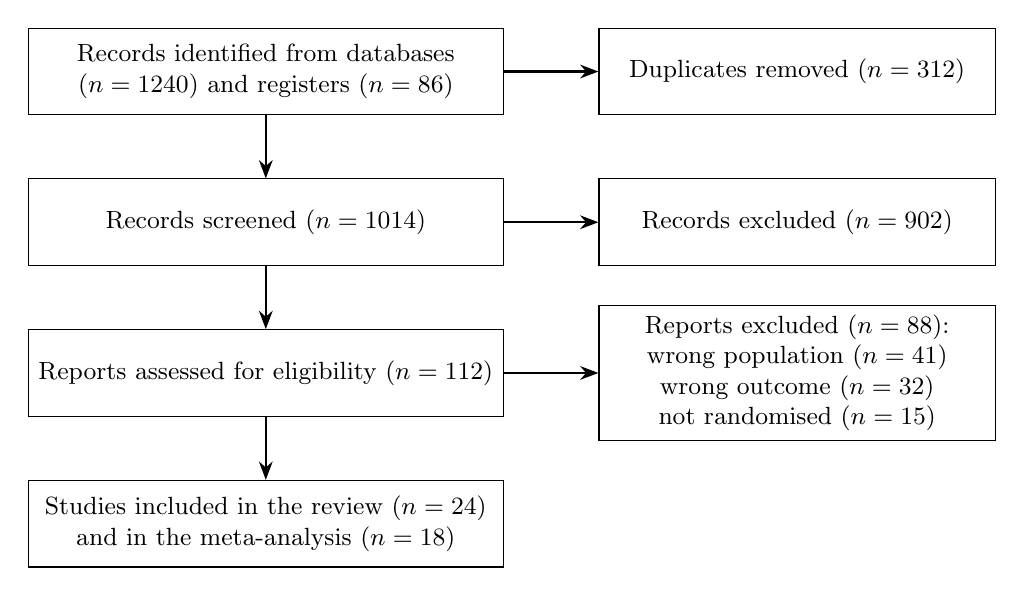
\begin{tikzpicture}[
      box/.style={draw, rectangle, align=flush center, text width=5.8cm, minimum height=1.1cm, font=\small},
      side/.style={box, text width=4.8cm},
      arrow/.style={-{Stealth}, thick},
      node distance=0.8cm and 1.2cm]
    \node[box] (id) {Records identified from databases ($n=1240$) and registers ($n=86$)};
    \node[side, right=of id] (dup) {Duplicates removed ($n=312$)};
    \node[box, below=of id] (screen) {Records screened ($n=1014$)};
    \node[side, right=of screen] (excl1) {Records excluded ($n=902$)};
    \node[box, below=of screen] (full) {Reports assessed for eligibility ($n=112$)};
    \node[side, right=of full] (excl2) {Reports excluded ($n=88$):\\ wrong population ($n=41$)\\ wrong outcome ($n=32$)\\ not randomised ($n=15$)};
    \node[box, below=of full] (incl) {Studies included in the review ($n=24$)\\ and in the meta-analysis ($n=18$)};
    \draw[arrow] (id) -- (screen);
    \draw[arrow] (screen) -- (full);
    \draw[arrow] (full) -- (incl);
    \draw[arrow] (id) -- (dup);
    \draw[arrow] (screen) -- (excl1);
    \draw[arrow] (full) -- (excl2);
  \end{tikzpicture}
  \caption{PRISMA 2020 flow diagram of the selection of studies.}
  \label{fig:prisma}
\end{figure}

\subsection{Study characteristics}
Table~\ref{tab:studies} summarises the included studies.

\begin{table}[htbp]
  \centering
  \caption{Characteristics of the included studies.}
  \label{tab:studies}
  \begin{tabular}{llrll}
    \toprule
    Study & Country & Participants & Follow-up & Risk of bias \\
    \midrule
    Study A 2019 & Country & 240 & 12 months & Low \\
    Study B 2021 & Country & 118 & 6 months & Some concerns \\
    Study C 2023 & Country & 412 & 24 months & Low \\
    \bottomrule
  \end{tabular}
\end{table}

\subsection{Results of syntheses}
Give the pooled estimates, heterogeneity and the certainty of the evidence.
A forest plot goes here.

\section{Discussion}
Summarise the evidence, compare it with earlier reviews, and discuss the
limitations of the studies and of the review.

\section{Conclusions}
State what the evidence means for practice and for research.

\section*{Declarations}
\subsection*{Registration and protocol}
Registry, number, and where the protocol can be read.

\subsection*{Funding}
List the funders and grant numbers, and their role in the review.

\subsection*{Competing interests}
The authors declare no competing interests.

\subsection*{Data availability}
The extracted data and analysis code are available in the supplement.

\subsection*{Reporting checklist}
The completed PRISMA 2020 checklist is provided as a supplementary file.

\bibliographystyle{vancouver}
\bibliography{references}

\end{document}
